%        File: DesignDocument.tex
%     Created: 一 3月 26 01:00 下午 2018 C
% Last Change: 一 3月 26 01:00 下午 2018 C
%
\documentclass[UTF8,noindent]{ctexart}
\usepackage[a4paper,left=2.0cm,right=2.0cm,top=2.0cm,bottom=2.0cm]{geometry}
\usepackage{hyperref}
\usepackage{url}
\usepackage{graphicx}
\usepackage{amsmath}
\usepackage{amssymb}
\usepackage{enumitem}
\usepackage{tikz}
\usepackage{float}
\usepackage{xeCJK}
\usepackage{listings}
\usepackage{xcolor}
\lstset{language = c,numbers=left, showstringspaces=false,keywordstyle= \color{ blue!70 },commentstyle=\color{red!50!green!50!blue!50}, frame=shadowbox, rulesepcolor= \color{ red!20!green!20!blue!20 } 
} 
\CTEXsetup[format={\Large\bfseries}]{section}
\usetikzlibrary{graphs}
%\newtheorem*{lemma}{Lemma}
\title{\CJKfamily{zhkai}计算机网络研讨课实验报告}
\author{{\CJKfamily{zhkai}冯吕}\ $2015K8009929049$}
\date{\today}
\begin{document}
\maketitle
\zihao{5}
\CJKfamily{zhsong}
%\begin{center}
%  \begin{tabular}{|p{15cm}|}
%    \hline
\section*{{\CJKfamily{zhhei}实验题目}}网络地址转换实验
%\hline
\section*{{\CJKfamily{zhhei}实验内容}}
本次实验需要实现$NAT$网络地址转换:
\begin{itemize}
  \item $NAT$映射表维护:维护$NAT$连接映射表,支持映射的添加、查找、更新和老化操作;
	\item 数据包的转换操作:
	  \begin{itemize}
		\item 对于到达的合法数据包,进行$IP$和$Port$转换操作,更新头部字段,并
转发数据包
\item 对于到达的非法数据包,回复$ICMP\ Destination\ Host\ Unreachable$
	  \end{itemize}
\end{itemize}

之后,根据给定网络拓扑,在$n1$上执行$nat$程序,在$h2$上运行$HTTP$服务,在$h1$上访问$h2$的$HTTP$服务。
\section*{{\CJKfamily{zhhei}实验流程}}
本次实验中,首先要实现$NAT$地址转换,主要需要事项三个函数:

$get\_packet\_direction(char *packet)$:该函数用于判断数据包的方向:尽或者热出。$nat$结构中存储有外部端口和内部端口的信息,因此,可根据数据包的源端口和目的端口来判断数据包的方向,如果数据包的源端口等于$nat$的内部端口并且目的端口等于$nat$的外部端口,那么则说明数据包是出去的;如果源端口等于$nat$的外部端口并且目的$ip$等于外部端口的$ip$,则说明是进来;否则为无效。
\begin{lstlisting}
static int get_packet_direction(char *packet)
{
	struct iphdr *ip_hdr = packet_to_ip_hdr(packet);
	rt_entry_t *src_entry = longest_prefix_match(ntohl(ip_hdr->saddr));
	rt_entry_t *dest_entry = longest_prefix_match(ntohl(ip_hdr->daddr));
	if(src_entry->iface == nat.internal_iface 
	&& dest_entry->iface == nat.external_iface){
		return DIR_OUT;
	}
	else if(src_entry->iface == nat.external_iface 
	&& ntohl(ip_hdr->daddr) == nat.external_iface->ip){
		return DIR_IN;
	}
	return DIR_INVALID;
}
\end{lstlisting}

$do\_translation$:该函数完成数据包的转换。首先判断数据包的方向,如果是出去,那么查找是否已经存在映射,如果不存在,则建立映射,然后更新头部字段,将包转发出去;如果包是进来,那么直接查找映射,然后更新头部信息,转发数据包,如果查找失败,则回复$ICMP$目的主机不可达消息。
\begin{lstlisting}
void do_translation(iface_info_t *iface, char *packet, int len, int dir)
{
	pthread_mutex_lock(&nat.lock);
	struct iphdr *ip = packet_to_ip_hdr(packet);
	struct tcphdr *tcp = packet_to_tcp_hdr(packet);
	int is_find = 0;
	struct nat_mapping  *nat_entry = NULL;
	u32 dest = ntohl(ip->daddr);
	u32 src = ntohl(ip->saddr);
	u16 sport = ntohs(tcp->sport);
	u16 dport = ntohs(tcp->dport);
	if(dir == DIR_IN){
		struct list_head *nat_entry_list = 
		&nat.nat_mapping_list[hash8((char*)&src,4)];
		if(!list_empty(nat_entry_list)){
			list_for_each_entry(nat_entry, 
			nat_entry_list, list){
				if(nat_entry->external_ip == dest 
				&& nat_entry->external_port == dport){
					is_find = 1;
					break;
				}
			}
		}
		if(!is_find){
			icmp_send_packet(packet, len, ICMP_DEST_UNREACH, 
			ICMP_HOST_UNREACH);
			free(packet);
		}
		else{
			ip->daddr = htonl(nat_entry->internal_ip);
			ip->checksum = ip_checksum(ip);
			tcp->dport = htons(nat_entry->internal_port);
			tcp->checksum = tcp_checksum(ip,tcp);
			nat_entry->update_time = time(NULL);
		}
	}
	else{
		struct list_head *nat_entry_list = 
		&nat.nat_mapping_list[hash8((char*)&dest,4)];
		if(!list_empty(nat_entry_list)){
			list_for_each_entry(nat_entry, nat_entry_list, list){
				if(nat_entry->internal_ip == src 
				&& nat_entry->internal_port == sport){
					is_find = 1;
					break;
				}
			}
		}
		if(!is_find){
			nat_entry = insert_nat_entry(src,
			sport,dest,nat_entry_list);
		}
		ip->saddr = htonl(nat_entry->external_ip);
		ip->checksum = ip_checksum(ip);
		tcp->sport = htons(nat_entry->external_port);
		tcp->checksum = tcp_checksum(ip,tcp);
		nat_entry->update_time = time(NULL);
	}
	ip_send_packet(packet,len);
	pthread_mutex_unlock(&nat.lock);
}
\end{lstlisting}

同时,$nat$还要不断进行老化操作:$nat\_timeout$。如果双方都已经发送$FIN$并回收$ACK$信息,则进行回收;如果已经超过$60s$没有发送数据,那么也认为传输结束,进行回收。
\begin{lstlisting}
void *nat_timeout()
{
	while (1) {
		sleep(1);
		struct nat_mapping  *nat_entry = NULL;
		struct nat_mapping  *nat_entry_next = NULL;
		pthread_mutex_lock(&nat.lock);
		for(int i =0; i < HASH_8BITS;i ++){
			struct list_head *nat_entry_list = 
			&nat.nat_mapping_list[i];
			if(list_empty(nat_entry_list))  
			  continue;
			list_for_each_entry_safe(nat_entry, nat_entry_next,
			nat_entry_list, list){
				if(nat_entry->conn.external_fin == 1 && 
			      nat_entry->conn.internal_fin == 1 && 
				  nat_entry->conn.external_seq_end == 
				  nat_entry->conn.internal_ack &&
		 		  nat_entry->conn.internal_seq_end == 
				  nat_entry->conn.external_ack){
					list_delete_entry(&nat_entry->list);
					free(nat_entry);
				}
				else if(time(NULL) - nat_entry->update_time
				> TCP_ESTABLISHED_TIMEOUT){
					list_delete_entry(&nat_entry->list);
					free(nat_entry);
				}
			}
		}
		pthread_mutex_unlock(&nat.lock);
	}

	return NULL;
}
\end{lstlisting}

实现$NAT$转换之后,根据给定拓扑进行网络服务实验。
\section*{{\CJKfamily{zhhei}实验结果}}
通过$h1$能够成功访问$h2$上的$HTTP$服务:
\begin{figure}[H]
  \centering
  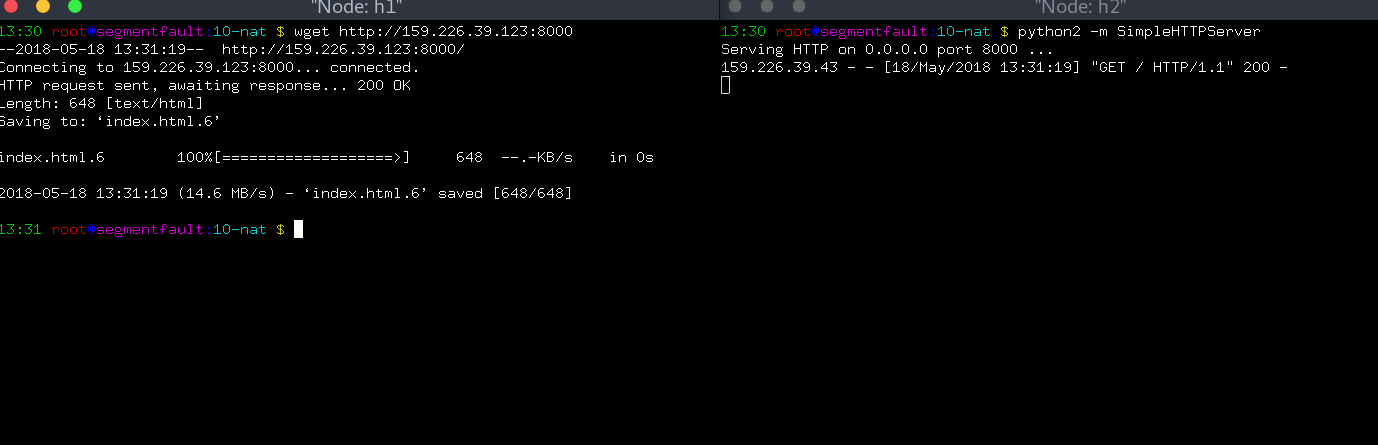
\includegraphics[scale=0.3]{1.png}
\end{figure}
\section*{{\CJKfamily{zhhei}结果分析}}
实验结果正确,$NAT$能够正确实现映射表的管理和数据包的转换。
\end{document}


